\documentclass{article}

\usepackage{tikz}
\usetikzlibrary{calc}
\begin{document}
\begin{figure}
\tikzset{
tick/.style = {black, very thick}
}

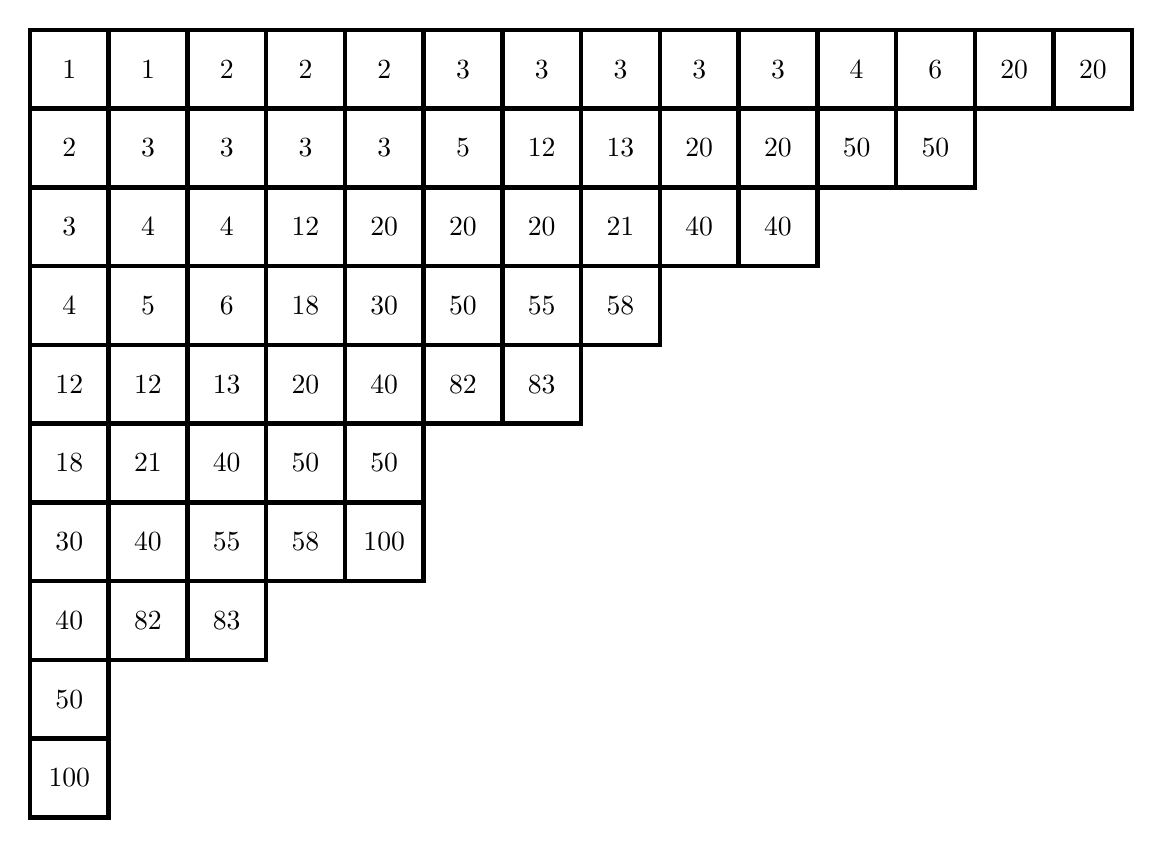
\begin{tikzpicture} % boxlength=1%ZEILE NR. 0 (von unten)

%ELEMENT IN SPALTE NR. 0 (von links)
\draw [ultra thick] (0,0) rectangle (1,1);
\node at ($(0.5,0.5)$) {$100$};




%ZEILE NR. 1 (von unten)

%ELEMENT IN SPALTE NR. 0 (von links)
\draw [ultra thick] (0,1) rectangle (1,2);
\node at ($(0.5,1.5)$) {$50$};




%ZEILE NR. 2 (von unten)

%ELEMENT IN SPALTE NR. 0 (von links)
\draw [ultra thick] (0,2) rectangle (1,3);
\node at ($(0.5,2.5)$) {$40$};

%ELEMENT IN SPALTE NR. 1 (von links)
\draw [ultra thick] (1,2) rectangle (2,3);
\node at ($(1.5,2.5)$) {$82$};

%ELEMENT IN SPALTE NR. 2 (von links)
\draw [ultra thick] (2,2) rectangle (3,3);
\node at ($(2.5,2.5)$) {$83$};




%ZEILE NR. 3 (von unten)

%ELEMENT IN SPALTE NR. 0 (von links)
\draw [ultra thick] (0,3) rectangle (1,4);
\node at ($(0.5,3.5)$) {$30$};

%ELEMENT IN SPALTE NR. 1 (von links)
\draw [ultra thick] (1,3) rectangle (2,4);
\node at ($(1.5,3.5)$) {$40$};

%ELEMENT IN SPALTE NR. 2 (von links)
\draw [ultra thick] (2,3) rectangle (3,4);
\node at ($(2.5,3.5)$) {$55$};

%ELEMENT IN SPALTE NR. 3 (von links)
\draw [ultra thick] (3,3) rectangle (4,4);
\node at ($(3.5,3.5)$) {$58$};

%ELEMENT IN SPALTE NR. 4 (von links)
\draw [ultra thick] (4,3) rectangle (5,4);
\node at ($(4.5,3.5)$) {$100$};




%ZEILE NR. 4 (von unten)

%ELEMENT IN SPALTE NR. 0 (von links)
\draw [ultra thick] (0,4) rectangle (1,5);
\node at ($(0.5,4.5)$) {$18$};

%ELEMENT IN SPALTE NR. 1 (von links)
\draw [ultra thick] (1,4) rectangle (2,5);
\node at ($(1.5,4.5)$) {$21$};

%ELEMENT IN SPALTE NR. 2 (von links)
\draw [ultra thick] (2,4) rectangle (3,5);
\node at ($(2.5,4.5)$) {$40$};

%ELEMENT IN SPALTE NR. 3 (von links)
\draw [ultra thick] (3,4) rectangle (4,5);
\node at ($(3.5,4.5)$) {$50$};

%ELEMENT IN SPALTE NR. 4 (von links)
\draw [ultra thick] (4,4) rectangle (5,5);
\node at ($(4.5,4.5)$) {$50$};




%ZEILE NR. 5 (von unten)

%ELEMENT IN SPALTE NR. 0 (von links)
\draw [ultra thick] (0,5) rectangle (1,6);
\node at ($(0.5,5.5)$) {$12$};

%ELEMENT IN SPALTE NR. 1 (von links)
\draw [ultra thick] (1,5) rectangle (2,6);
\node at ($(1.5,5.5)$) {$12$};

%ELEMENT IN SPALTE NR. 2 (von links)
\draw [ultra thick] (2,5) rectangle (3,6);
\node at ($(2.5,5.5)$) {$13$};

%ELEMENT IN SPALTE NR. 3 (von links)
\draw [ultra thick] (3,5) rectangle (4,6);
\node at ($(3.5,5.5)$) {$20$};

%ELEMENT IN SPALTE NR. 4 (von links)
\draw [ultra thick] (4,5) rectangle (5,6);
\node at ($(4.5,5.5)$) {$40$};

%ELEMENT IN SPALTE NR. 5 (von links)
\draw [ultra thick] (5,5) rectangle (6,6);
\node at ($(5.5,5.5)$) {$82$};

%ELEMENT IN SPALTE NR. 6 (von links)
\draw [ultra thick] (6,5) rectangle (7,6);
\node at ($(6.5,5.5)$) {$83$};




%ZEILE NR. 6 (von unten)

%ELEMENT IN SPALTE NR. 0 (von links)
\draw [ultra thick] (0,6) rectangle (1,7);
\node at ($(0.5,6.5)$) {$4$};

%ELEMENT IN SPALTE NR. 1 (von links)
\draw [ultra thick] (1,6) rectangle (2,7);
\node at ($(1.5,6.5)$) {$5$};

%ELEMENT IN SPALTE NR. 2 (von links)
\draw [ultra thick] (2,6) rectangle (3,7);
\node at ($(2.5,6.5)$) {$6$};

%ELEMENT IN SPALTE NR. 3 (von links)
\draw [ultra thick] (3,6) rectangle (4,7);
\node at ($(3.5,6.5)$) {$18$};

%ELEMENT IN SPALTE NR. 4 (von links)
\draw [ultra thick] (4,6) rectangle (5,7);
\node at ($(4.5,6.5)$) {$30$};

%ELEMENT IN SPALTE NR. 5 (von links)
\draw [ultra thick] (5,6) rectangle (6,7);
\node at ($(5.5,6.5)$) {$50$};

%ELEMENT IN SPALTE NR. 6 (von links)
\draw [ultra thick] (6,6) rectangle (7,7);
\node at ($(6.5,6.5)$) {$55$};

%ELEMENT IN SPALTE NR. 7 (von links)
\draw [ultra thick] (7,6) rectangle (8,7);
\node at ($(7.5,6.5)$) {$58$};




%ZEILE NR. 7 (von unten)

%ELEMENT IN SPALTE NR. 0 (von links)
\draw [ultra thick] (0,7) rectangle (1,8);
\node at ($(0.5,7.5)$) {$3$};

%ELEMENT IN SPALTE NR. 1 (von links)
\draw [ultra thick] (1,7) rectangle (2,8);
\node at ($(1.5,7.5)$) {$4$};

%ELEMENT IN SPALTE NR. 2 (von links)
\draw [ultra thick] (2,7) rectangle (3,8);
\node at ($(2.5,7.5)$) {$4$};

%ELEMENT IN SPALTE NR. 3 (von links)
\draw [ultra thick] (3,7) rectangle (4,8);
\node at ($(3.5,7.5)$) {$12$};

%ELEMENT IN SPALTE NR. 4 (von links)
\draw [ultra thick] (4,7) rectangle (5,8);
\node at ($(4.5,7.5)$) {$20$};

%ELEMENT IN SPALTE NR. 5 (von links)
\draw [ultra thick] (5,7) rectangle (6,8);
\node at ($(5.5,7.5)$) {$20$};

%ELEMENT IN SPALTE NR. 6 (von links)
\draw [ultra thick] (6,7) rectangle (7,8);
\node at ($(6.5,7.5)$) {$20$};

%ELEMENT IN SPALTE NR. 7 (von links)
\draw [ultra thick] (7,7) rectangle (8,8);
\node at ($(7.5,7.5)$) {$21$};

%ELEMENT IN SPALTE NR. 8 (von links)
\draw [ultra thick] (8,7) rectangle (9,8);
\node at ($(8.5,7.5)$) {$40$};

%ELEMENT IN SPALTE NR. 9 (von links)
\draw [ultra thick] (9,7) rectangle (10,8);
\node at ($(9.5,7.5)$) {$40$};




%ZEILE NR. 8 (von unten)

%ELEMENT IN SPALTE NR. 0 (von links)
\draw [ultra thick] (0,8) rectangle (1,9);
\node at ($(0.5,8.5)$) {$2$};

%ELEMENT IN SPALTE NR. 1 (von links)
\draw [ultra thick] (1,8) rectangle (2,9);
\node at ($(1.5,8.5)$) {$3$};

%ELEMENT IN SPALTE NR. 2 (von links)
\draw [ultra thick] (2,8) rectangle (3,9);
\node at ($(2.5,8.5)$) {$3$};

%ELEMENT IN SPALTE NR. 3 (von links)
\draw [ultra thick] (3,8) rectangle (4,9);
\node at ($(3.5,8.5)$) {$3$};

%ELEMENT IN SPALTE NR. 4 (von links)
\draw [ultra thick] (4,8) rectangle (5,9);
\node at ($(4.5,8.5)$) {$3$};

%ELEMENT IN SPALTE NR. 5 (von links)
\draw [ultra thick] (5,8) rectangle (6,9);
\node at ($(5.5,8.5)$) {$5$};

%ELEMENT IN SPALTE NR. 6 (von links)
\draw [ultra thick] (6,8) rectangle (7,9);
\node at ($(6.5,8.5)$) {$12$};

%ELEMENT IN SPALTE NR. 7 (von links)
\draw [ultra thick] (7,8) rectangle (8,9);
\node at ($(7.5,8.5)$) {$13$};

%ELEMENT IN SPALTE NR. 8 (von links)
\draw [ultra thick] (8,8) rectangle (9,9);
\node at ($(8.5,8.5)$) {$20$};

%ELEMENT IN SPALTE NR. 9 (von links)
\draw [ultra thick] (9,8) rectangle (10,9);
\node at ($(9.5,8.5)$) {$20$};

%ELEMENT IN SPALTE NR. 10 (von links)
\draw [ultra thick] (10,8) rectangle (11,9);
\node at ($(10.5,8.5)$) {$50$};

%ELEMENT IN SPALTE NR. 11 (von links)
\draw [ultra thick] (11,8) rectangle (12,9);
\node at ($(11.5,8.5)$) {$50$};




%ZEILE NR. 9 (von unten)

%ELEMENT IN SPALTE NR. 0 (von links)
\draw [ultra thick] (0,9) rectangle (1,10);
\node at ($(0.5,9.5)$) {$1$};

%ELEMENT IN SPALTE NR. 1 (von links)
\draw [ultra thick] (1,9) rectangle (2,10);
\node at ($(1.5,9.5)$) {$1$};

%ELEMENT IN SPALTE NR. 2 (von links)
\draw [ultra thick] (2,9) rectangle (3,10);
\node at ($(2.5,9.5)$) {$2$};

%ELEMENT IN SPALTE NR. 3 (von links)
\draw [ultra thick] (3,9) rectangle (4,10);
\node at ($(3.5,9.5)$) {$2$};

%ELEMENT IN SPALTE NR. 4 (von links)
\draw [ultra thick] (4,9) rectangle (5,10);
\node at ($(4.5,9.5)$) {$2$};

%ELEMENT IN SPALTE NR. 5 (von links)
\draw [ultra thick] (5,9) rectangle (6,10);
\node at ($(5.5,9.5)$) {$3$};

%ELEMENT IN SPALTE NR. 6 (von links)
\draw [ultra thick] (6,9) rectangle (7,10);
\node at ($(6.5,9.5)$) {$3$};

%ELEMENT IN SPALTE NR. 7 (von links)
\draw [ultra thick] (7,9) rectangle (8,10);
\node at ($(7.5,9.5)$) {$3$};

%ELEMENT IN SPALTE NR. 8 (von links)
\draw [ultra thick] (8,9) rectangle (9,10);
\node at ($(8.5,9.5)$) {$3$};

%ELEMENT IN SPALTE NR. 9 (von links)
\draw [ultra thick] (9,9) rectangle (10,10);
\node at ($(9.5,9.5)$) {$3$};

%ELEMENT IN SPALTE NR. 10 (von links)
\draw [ultra thick] (10,9) rectangle (11,10);
\node at ($(10.5,9.5)$) {$4$};

%ELEMENT IN SPALTE NR. 11 (von links)
\draw [ultra thick] (11,9) rectangle (12,10);
\node at ($(11.5,9.5)$) {$6$};

%ELEMENT IN SPALTE NR. 12 (von links)
\draw [ultra thick] (12,9) rectangle (13,10);
\node at ($(12.5,9.5)$) {$20$};

%ELEMENT IN SPALTE NR. 13 (von links)
\draw [ultra thick] (13,9) rectangle (14,10);
\node at ($(13.5,9.5)$) {$20$};







\end{tikzpicture}
\end{figure}
\end{document}

